\documentclass[main.tex]{subfile}

\begin{document}

\section{Nyquist Frequency} 
\label{sec:nyquist_frequency}

A given sinusoidal wave is represented mathematically as:

\begin{align}
  x(t) = A\sin{((\omega t + \phi))} + y
\end{align}
where $A$ is the amplitude, $\omega$ is the angular frequency, $\phi$ is the
phase shift, and $y$ is the y-axis offset. If an Analog-to-Digital-Converter (or
ADC) circuit is used to obtain a digital representation of the signal we then
have the corresponding digital sinusoidal wave: 

\begin{align}
  x[n] = A\sin{(\omega \delta_{t} n + \phi)} + y \label{eq:sampledWave}
\end{align}
where $n$ is the n$^{th}$ sample and $\delta_{t}$ is the sampling time step size
which is obtained from the sampling frequency $f_s$ as $\delta_{t} =
\frac{1}{f_s}$. If the sampling frequency is lower than the frequency of the
wave being sampled then the aliasing affect occurs as follows.

First we observe that a sin wave is periodic every $2\pi$ and thus phase shifts
of $2\pi a$ have no change on the wave form. Applying this principle to \eqref{sampledWave}
we obtain the following:

\begin{align}
  x[n] &= A\sin{(2\pi f \delta_{t} n + \phi)} + y \label{eq:sampledWave}
  \\&= A\sin{(2\pi f \delta_{t} n + 2\pi a + \phi)} + y
  \\&= A\sin{(2\pi \delta_{t} n (f + )}) + y
\end{align}

$f + \frac{a}{n\delta_{t}}$ is known as the alias frequency as it creates a different
sinusoidal wave than above but with the same sampled data.

% section nyquist_frequency (end)

\begin{figure}[H]
  \begin{center}
    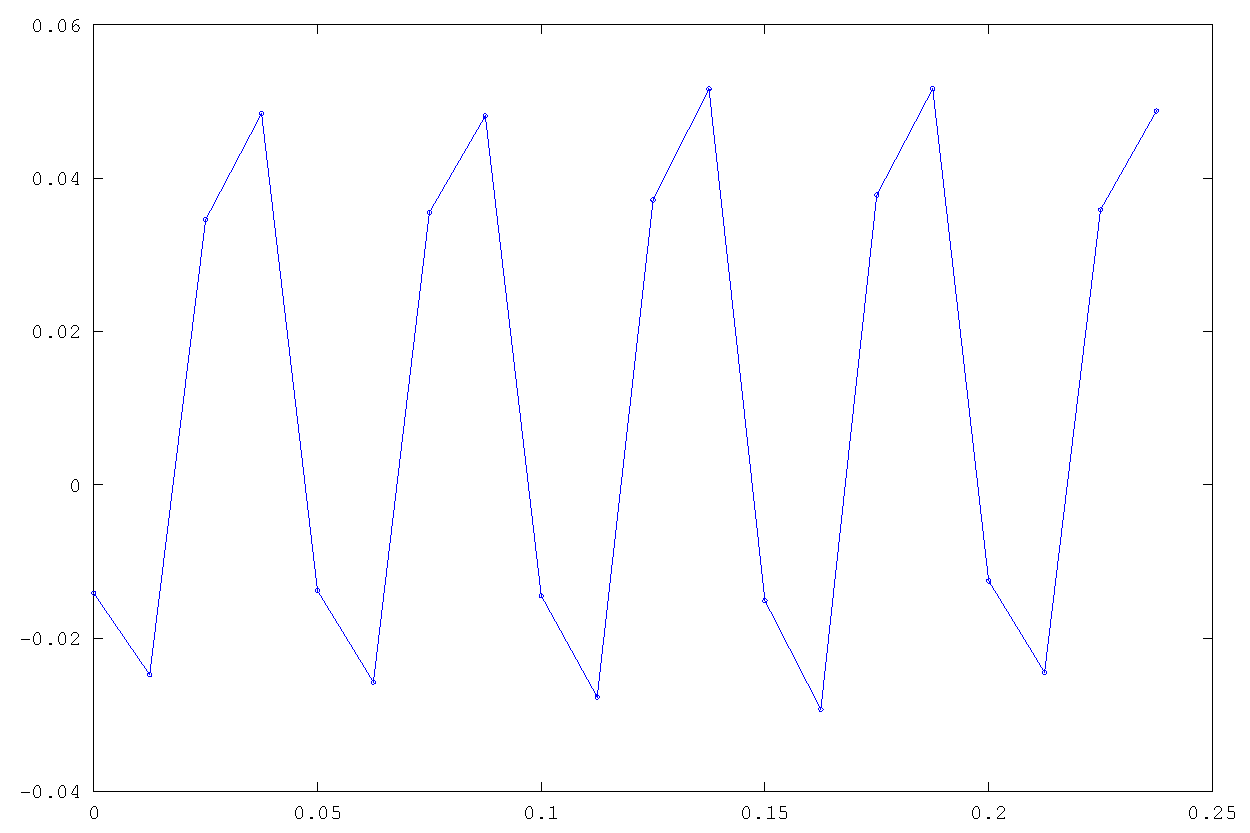
\includegraphics[width=\linewidth]{pt2_80Hz.pdf}
  \end{center}
  \caption{$80\dem{Hz}$ Measured Sine Wave}
  \label{fig:pt280hz}
\end{figure}

Following simulation, the experiment continued with analysis of physical
electrical frequencies using the ELVIS II board as a function generator and
LabVIEW as a digital acquisition device (DAQ). The function generator on the
ELVIS board was configured to generate a 100 Hz sine wave with a 0.1 volt
peak-to-peak amplitude. The function generator was then wired to the analog
input channel on the same board. In LabView a DAQ assistant block was placed
and set to measure voltage on the same analog input channel. The DAQ was then
configured to take 8 samples in the range of -10 to 10 volts; 8 samples is
sufficient to capture 10 periods of the 100 Hz wave at a sample rate of 80 Hz.
The data was exported to an Excel spreadsheet and differences between the
sampled waveform and an ideal sine wave were noted.  

The sample rate was then increased to 200 Hz and the waveform was then
re-sampled, using enough samples to capture 10 periods of the source wave. As in
the previous test, the sampled data were recorded to a spreadsheet and the
differences between the sample data and an ideal sine wave were noted.

\begin{figure}[H]
  \begin{center}
    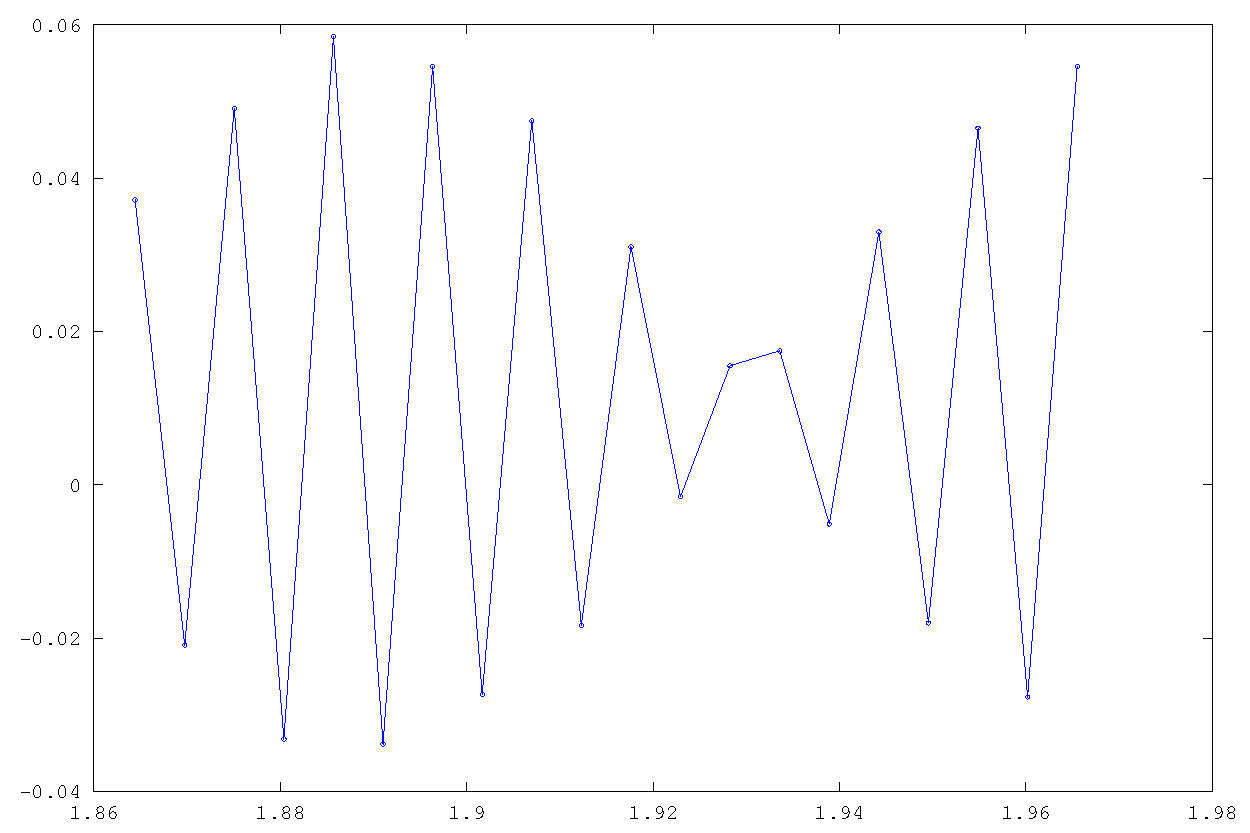
\includegraphics[width=\linewidth]{pt2_200Hz.pdf}
  \end{center}
  \caption{$200\dem{Hz}$ Measured Sine Wave}
  \label{fig:pt280hz}
\end{figure}
% document text goes here

Notice that the higher sampling rate gives a more accurate representation of the
generated sinusoidal wave. A attribute what appears to be modulation in the amplitude
of \figref{pt280hz} to the fact that even at a higher sampling rate not enough
data is gathered in a single period of the sampled wave to avoid missing pieces
of data.

\end{document}
